\documentclass[12pt]{article}

%-------------------------------------------------
% PAGE & LANGUAGE
% -------------------------------------------------

\usepackage[a4paper,margin=2cm]{geometry}

% -------------------------------------------------
% MATHEMATICS
% -------------------------------------------------

\usepackage{amsmath}
\usepackage{amssymb}
\usepackage{amsthm}
\usepackage{mathtools}
\usepackage{yhmath}

% Physics notation
\usepackage{physics}

% -------------------------------------------------
% GRAPHICS & PLOTS
% -------------------------------------------------

\usepackage{graphicx}
\usepackage{tikz}
\usetikzlibrary{3d,arrows.meta}
\usepackage{pgfplots}

\pgfplotsset{compat=1.18}
\graphicspath{{./images/}}

% -------------------------------------------------
% COLORS & BOXES
% -------------------------------------------------

\usepackage[dvipsnames,svgnames,x11names]{xcolor}
\usepackage{tcolorbox}
\tcbuselibrary{skins,breakable}
\newtcolorbox{demobox}[1][]{
    enhanced,
    breakable,
    colback=black!2,
    colframe=black!70,
    boxrule=0pt,
    borderline west={2pt}{0pt}{black!70},
    sharp corners,
    left=10pt,
    right=7pt,
    top=6pt,
    bottom=6pt,
    fonttitle=\bfseries,
    title={Demostració},
    #1
}

\newtcolorbox{examplebox}[1]{
    enhanced,
    breakable,
    colback=black!1,
    colframe=black!15,
    boxrule=0.5pt,
    arc=2mm,
    borderline west={2pt}{0pt}{black!55},
    left=12pt,
    right=12pt,
    top=10pt,
    bottom=10pt,
    before skip=12pt,
    after skip=12pt,
    title={\textbf{Exemple #1}},
    fonttitle=\normalsize,
    coltitle=black,
    attach boxed title to top left={
        xshift=8pt,
        yshift=-\tcboxedtitleheight/2
    },
    boxed title style={
        colback=white,
        colframe=white,
        boxrule=0pt,
        left=3pt,
        right=3pt,
        top=1pt,
        bottom=1pt
    },
    before upper={\setlength{\parskip}{7pt}}
}

% -------------------------------------------------
% DOCUMENT FORMATTING
% -------------------------------------------------

\usepackage{enumitem}
\usepackage[expansion=false]{microtype}
\usepackage{booktabs}
\usepackage{float}
\usepackage{ragged2e}

% -------------------------------------------------
% CHEMISTRY
% -------------------------------------------------

\usepackage[version=4]{mhchem}

% -------------------------------------------------
% LINKS
% --------------------------------------------------

\usepackage[colorlinks=true,linkcolor=Black,urlcolor=Black,citecolor=Black]{hyperref}
\usepackage{tocloft}
\usepackage{cite}

% -------------------------------------------------
% CUSTOM COMMANDS
% -------------------------------------------------

\newcommand{\R}{\mathbb{R}}
\newcommand{\N}{\mathbb{N}}
\newcommand{\Z}{\mathbb{Z}}

% -------------------------------------------------
% DOCUMENT STYLE
% -------------------------------------------------

\linespread{1.25}

\setlength{\parskip}{0.8em}
\setlength{\parindent}{0pt}

\setlength{\heavyrulewidth}{0.4pt}
\setlength{\heavyrulewidth}{0.4pt}
\setlength{\lightrulewidth}{0.4pt}
\setlength{\cmidrulewidth}{0.4pt}

\title{\textbf{Apunts Mecànica, Ones i Relativitat}}
\author{\textit{Gerard Cosp Lores}}
\date{\today}

% -------------------------------------------------
% TABLE OF CONTENTS
% -------------------------------------------------

\renewcommand{\contentsname}{Índex}

% Title
\renewcommand{\cfttoctitlefont}{%
    \Huge\bfseries\color{Black}
}

% Line underneath title
\renewcommand{\cftaftertoctitle}{%
    \par\vspace{0.3cm}
    \noindent\color{Black}\rule{\textwidth}{1.2pt}
    \vspace{0.4cm}
}

% Section appearance
\renewcommand{\cftsecfont}{%
    \large\bfseries\color{Black}
}

\renewcommand{\cftsecpagefont}{%
    \large\bfseries\color{Black}
}

% Subsection appearance
\renewcommand{\cftsubsecfont}{%
    \normalsize
}

\renewcommand{\cftsubsecpagefont}{%
    \normalsize\color{Black}
}

% Spacing
\setlength{\cftbeforesecskip}{10pt}
\setlength{\cftbeforesubsecskip}{3pt}

% Dotted leaders
\renewcommand{\cftsecleader}{%
    \color{Black}\cftdotfill{\cftdotsep}
}

\renewcommand{\cftsubsecleader}{%
    \color{Black}\cftdotfill{\cftdotsep}
}

% Number spacing
\setlength{\cftsecnumwidth}{2.5em}
\setlength{\cftsubsecnumwidth}{3.5em}

% -------------------------------------------------

\begin{document}
\justifying

\maketitle
\tableofcontents

\newpage

\section{Cinemàtica (Descripció del moviment)}

Considerem una partícula puntual (0-D), la posició d'aquest punt la podem descriure com un vector en un eix 3-D ($\vec{r}$).

En qualsevol sistema de coordenades tenim els \textbf{vectors unitaris} són vectors que pertanyen al espai i defineixen la nostra base de manera que ($\abs{\vec{u_i}} = 1u$). En les nostres bases cartesianes tenim els vectors ($\vec{i}, \vec{j}, \vec{k}$) per tant podem descriure el \textit{vector posició} com

\[\vec{r} = x\vec{i} + y\vec{j} + z\vec{k}\]

\begin{center}
   \begin{tikzpicture}[>=Stealth, scale=1]
  \draw [<-](-0.2,2.2) -- (-0.2,-0.4);
  \draw [->](-0.2,-0.4) -- (2.6,-0.4);
  \node[
  % draw,
  inner sep=0pt,
  align=center,
  text=black
] at (-0.2,2.4) {z};
  \node[
  % draw,
  inner sep=0pt,
  align=center,
  text=black
] at (-1.2,-1.5) {x};
  \node[
  % draw,
  inner sep=0pt,
  align=center,
  text=black
] at (2.6,-0.2) {y};
  \node[inner sep=0pt, align=center, text=red!60!black, node font=\scriptsize, rotate=40] (node2) at (1.5,1.5) {$\vec{r}(t)$};
  \draw[arrows=-stealth, thick, red!60!black] (-0.2,-0.4) -- (2,1.52);
  \draw [<-](-1.08,-1.4) -- (1.2,1.2);
  \draw[->, green!60!black] (-0.2,-0.4) -- (-0.2,0.2);
\draw[->, yellow!60!black] (-0.2,-0.4) -- (-0.46,-0.69);
\draw[->, blue!60!black] (-0.2,-0.4) -- (0.29,-0.4);
\end{tikzpicture}
\end{center}

Quan algo es mou o canvia és degut al temps (esdevé funció del temps).

Per tant podem dir que;

\[\vec{r}(t) = x(t)\vec{i} + y(t)\vec{j} + z(t)\vec{k}\]

I anomenem a aquesta igualtat, \textbf{equació del moviment}.

\begin{examplebox}{1}
    Una particula descriu una corba $\vec{r}(t) = R\cos(\omega t)\vec{i} + R\sin(\omega t)\vec{j}$ si pensem una mica, \textbf{és un document en dos dimensions}. Per saber la trajectoria calculem $\abs{\vec{r}(t)}$ i amb l'identitat pitagòrica ens queda que la trajectoria respecte l'origen és $R^2$ que no és més que una constant.

    Si pensem encara una mica més la trajectoria constant i que sempre té la mateixa distàncai és la circular per tant aquella igualtat determina un \textbf{moviment circular}
\end{examplebox}

\subsection{Velocitats}

Quan hi ha un canvi en el temps i un canvi en la posició ($\Delta t, \Delta \vec{r}$) Apareix un vector $\vec{v}$ que també depèn de t i ens diu com ha canviar la posició en aquell temps. El vector apuntarà en direcció a la secant entre els vectors $\vec{r_0}, \vec{r_1}$ i és calcula de manera $v_m = \frac{\Delta \vec{r}}{\Delta t}$.

\begin{center}
    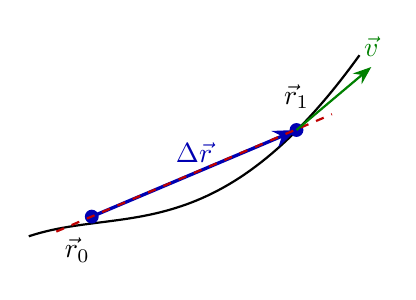
\begin{tikzpicture}[>=Stealth, scale=1]

    % Trajectòria
    \draw[
        thick,
        black
    ] (0,0.4)
    .. controls (1.2,0.8) and (2.4,0.2) ..
    (4.2,2.7);

    % Posicions
    \fill[blue!70!black] (0.8,0.65) circle (2.5pt);
    \fill[blue!70!black] (3.4,1.75) circle (2.5pt);

    \node[below left] at (0.9,0.5) {$\vec r_0$};
    \node[above] at (3.4,1.9) {$\vec r_1$};

    % Vector desplaçament
    \draw[
        ->,
        very thick,
        blue!70!black
    ] (0.8,0.65) -- (3.4,1.75)
        node[midway, above] {$\Delta\vec r$};

    % Secant
    \draw[
        dashed,
        red!75!black,
        thick
    ] (0.35,0.46) -- (3.85,1.95)
        node[midway, below] {\color{red!75!black}};

    % Tangent aproximada
    \draw[
        ->,
        thick,
        green!50!black
    ] (3.4,1.75) -- (4.35,2.55)
        node[above] {\color{green!50!black}$\vec v$};

    \end{tikzpicture}
\end{center}

Ara. \textbf{I si fem aquest intèrval $\Delta t$ infinitéssimament petit?} és a dir plantejem el límit.

$\vec{v}(t) \equiv \lim_{\Delta t \rightarrow 0} \frac{\Delta \vec{r}}{\Delta t} = \dot{\vec{r}}(t)$

Que bàsicament ens dona el canvi de posició respeccte el petitíssim canvi de temps, donant així una \textbf{velocitat instantània}. Com que aquesta fa que l'intèrval de $\vec{r}(t)$ estigui més junt, el vector velocitat passa a \textit{ser tangent a la trajectoria}.

\begin{center}
    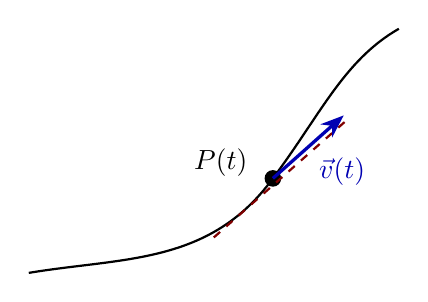
\begin{tikzpicture}[>=Stealth, scale=1]

    % Trajectòria
    \draw[
        thick,
        black
    ] (0,0.3)
    .. controls (1.2,0.5) and (2.3,0.4) ..
    (3.1,1.5)
    .. controls (3.7,2.3) and (4.0,3.0) ..
    (4.7,3.4);

    % Punt instantani
    \fill[black] (3.1,1.5) circle (3pt);
    \node[left] at (2.9,1.7) {$P(t)$};

    % Tangent
    \draw[
        dashed,
        red!50!black,
        thick
    ] (2.35,0.75) -- (4.05,2.25);

    % Velocitat
    \draw[
        ->,
        very thick,
        blue!70!black
    ] (3.1,1.5) -- (4.0,2.3)
        node[midway, below right] {$\vec v(t)$};


    \end{tikzpicture}
\end{center}

Parlem de \textbf{celeritat o rapidesa} quan fem el mòdul del vector velocitat.

\[\dot{\vec{r}}(t) = \dot{x}(t)\vec{i} + \dot{y}(t)\vec{j} + \dot{z}(t)\vec{k}\]

\subsection{Acceleracions}

Quan hi ha un canvi en el temps i un canvi en la velocitat ($\Delta t, \Delta \dot{\vec{r}}$) Apareix un vector $\vec{a}$ que també depèn de t i ens diu com ha canviar la velocitat en aquell temps. El vector no sempre apuntarà en direcció a la secant entre els vectors $\dot{\vec{r_0}}, \dot{\vec{r_1}}$ i és calcula de manera $a_m = \frac{\Delta \dot{\vec{r}}}{\Delta t}$.

\begin{center}
    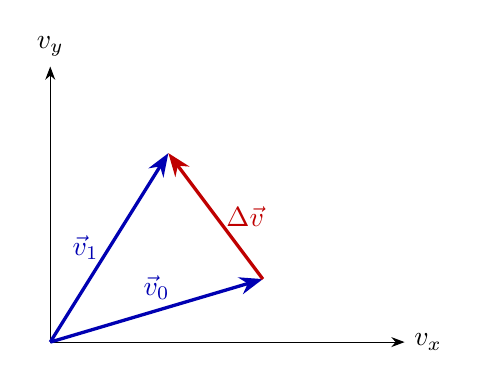
\begin{tikzpicture}[>=Stealth, scale=1]

    % Espai de velocitats
    \draw[->, black] (0,0) -- (4.5,0)
        node[right] {$v_x$};
    \draw[->, black] (0,0) -- (0,3.5)
        node[above] {$v_y$};

    % v0
    \draw[
        ->,
        very thick,
        blue!70!black
    ] (0,0) -- (2.7,0.8)
        node[midway, above] {$\vec v_0$};

    % v1
    \draw[
        ->,
        very thick,
        blue!70!black
    ] (0,0) -- (1.5,2.4)
        node[midway, left] {$\vec v_1$};

    % Delta v
    \draw[
        ->,
        very thick,
        red!75!black
    ] (2.7,0.8) -- (1.5,2.4)
        node[midway, right] {$\Delta\vec v$};

    \end{tikzpicture}
\end{center}

Ara. \textbf{I si fem aquest intèrval $\Delta t$ infinitéssimament petit?} és a dir plantejem el límit.

$\vec{a}(t) \equiv \lim_{\Delta t \rightarrow 0} \frac{\Delta \dot{\vec{r}}}{\Delta t} = \ddot{\vec{r}}(t)$

Que bàsicament ens dona el canvi de velocitat respeccte el petitíssim canvi de temps, donant així una \textbf{acceleració instantània}. Aquest vector $\vec{a}$ no ha d'apuntar a la tangent de trajectoria, de fet apunta a la tangent de velocitat i el seu sentit és totalment arbitrari. Podem \textbf{desglossar} l'acceleració (al igual que fem amb les components d'una força) en \textit{$a_t$} que és l'acceleració tangencial que segueix la tangent del moviment i \textit{$a_n$} que és la normal que forma un angle de $\frac{\pi}{2}rad$ amb la tangencial.

\begin{center}

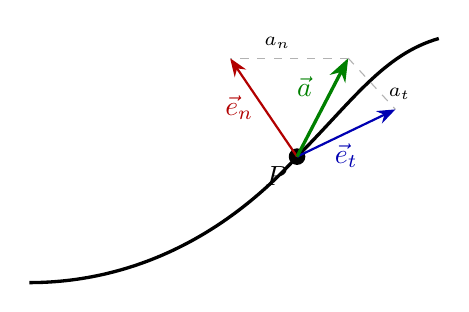
\begin{tikzpicture}[>=Stealth, scale=1]

% Trajectòria
\draw[
    very thick,
    black
] (0,0.3)
  .. controls (1.2,0.3) and (2.4,0.8) ..
  (3.4,1.9)
  .. controls (4.1,2.6) and (4.5,3.2) ..
  (5.2,3.4);

% Punt P
\fill (3.4,1.9) circle (3pt);
\node[below left] at (3.4,1.9) {$P$};

% Vector tangent
\draw[
    ->,
    thick,
    blue!70!black
] (3.4,1.9) -- (4.65,2.5)
    node[midway, below] {$\vec e_t$};

% Vector normal (perpendicular)
\draw[
    ->,
    thick,
    red!70!black
] (3.4,1.9) -- (2.55,3.15)
    node[midway, left] {$\vec e_n$};

% Acceleració
\draw[
    ->,
    very thick,
    green!50!black
] (3.4,1.9) -- (4.05,3.15)
    node[midway, above left] {$\vec a$};

% Triangle de components
\draw[
    dashed,
    gray!60
] (4.05,3.15) -- (4.65,2.5);

\draw[
    dashed,
    gray!60
] (4.05,3.15) -- (2.55,3.15);

% Components
\node at (4.7,2.7) {\scriptsize $a_t$};
\node at (3.15,3.35) {\scriptsize $a_n$};

\end{tikzpicture}

\end{center}
\[\ddot{\vec{r}}(t) = \ddot{x}(t)\vec{i} + \ddot{y}(t)\vec{j} + \ddot{z}(t)\vec{k}\]

\subsection{MRU (1-D)}

Parlem de MRU quan $\Delta v = 0$ és a dir que la velocitat és constant i que el canvi de posició és sempre el mateix.

\begin{center}
\begin{tikzpicture}[>=Stealth, scale=0.9]

% Eixos
\draw[->] (0,0) -- (5.2,0) node[right] {$t$};
\draw[->] (0,0) -- (0,3.5) node[above] {$x$};

% Recta MRU
\draw[
    very thick,
    blue!70!black
] (0.4,0.6) -- (4.7,3.0);

% Punts
\fill[red!70!black] (1.3,1.1) circle (2.5pt);
\fill[red!70!black] (2.7,1.9) circle (2.5pt);
\fill[red!70!black] (4.1,2.65) circle (2.5pt);

\end{tikzpicture}
\end{center}

Sabem que si $\dv{x}{t} = v \therefore dx = v\cdot dt \therefore \int dx = \int v dt \therefore x = k + vt$ i d'aquí surt que;

\[x(t) = x_0 + v(t-t_0)\]

\subsection{MRUA}

Aquí l'acceleració és constant per tant hem de trobar una expressió en funció del temps que ens descrigui la velocitat. Fent servir $\dv{v}{t} = a, \dv[2]{x}{t} = a$, obtenim;

\begin{center}
\begin{tikzpicture}[>=Stealth, scale=0.9]

% Eixos
\draw[->] (0,0) -- (5.2,0) node[right] {$t$};
\draw[->] (0,0) -- (0,3.5) node[above] {$v$};

% Recta v(t)
\draw[
    very thick,
    red!70!black
] (0.5,0.8) -- (4.6,3.0);

% Punts
\fill[blue!70!black] (1.3,1.2) circle (2.5pt);
\fill[blue!70!black] (3.7,2.55) circle (2.5pt);

\end{tikzpicture}
\end{center}

\begin{center}

\begin{tikzpicture}[>=Stealth, scale=0.9]

% Eixos

\draw[->] (0,0) -- (5.2,0) node[right] {$t$};

\draw[->] (0,0) -- (0,3.8) node[above] {$x$};

% Paràbola x(t)

\draw[
    very thick,
    red!70!black
] (0.5,0.6)
  .. controls (1.5,0.7) and (2.8,1.1) ..
  (4.6,3.2);

% Punts

\fill[blue!70!black] (1.3,0.75) circle (2.5pt);

\fill[blue!70!black] (3.7,2.25) circle (2.5pt);

\end{tikzpicture}

\end{center}

\[x(t) = x_0 + v(t-t_0) + \frac{1}{2}a(t-t_0)^2\]
\[v(t) = v_0 + a(t-t_0)\]

% equacio parabola

\subsection{Canvis en els sistemes de referència}

Podem escollir el nostre sistema de referència com vulguem pero estem \textbf{obligats a donar la referència}. Per crear el nostre sistema de referència fem ús de dos axiomes que no funcionen en la Relativitat d'Einstein; 

\begin{itemize}
    \item Axioma I: El temps és absolut (\textit{transcorre al mateix ritme per tothom})
    \item Axioma II: Espai absolut (\textit{Tot es troba al mateix espai})
\end{itemize}

Si definim 2 bases (R i R') que es diferencien pel vector que depèn del temps $\vec{R}(t)$, Per arribar al punt des de R fem servir el vector $\vec{r}$ i per arribar al punt des de R' fem servir $\vec{r'}$. Llavors podem definir $\vec{r}$ com $\vec{r} = \vec{R} + \vec{r'}$

\begin{center}
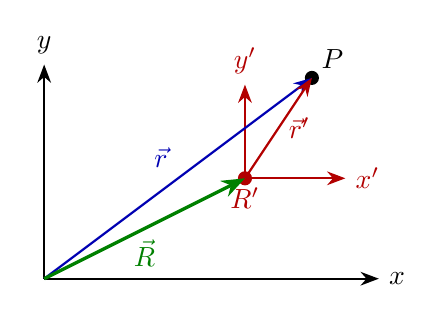
\begin{tikzpicture}[>=Stealth, scale=0.85]

% Sistema R
\draw[->, thick] (0,0) -- (5,0) node[right] {$x$};
\draw[->, thick] (0,0) -- (0,3.2) node[above] {$y$};

% Origen R'
\fill[red!70!black] (3,1.5) circle (3pt);
\node[red!70!black] [below] at (3,1.5) {$R'$};

% Eixos R'
\draw[->, red!70!black, thick]
    (3,1.5) -- (4.50,1.5)
    node[right] {$x'$};

\draw[->, red!70!black, thick]
    (3,1.5) -- (3, 2.9)
    node[above] {$y'$};

% Punt
\fill[black] (4.0,3) circle (3pt);
\node[above right] at (4.0,3) {$P$};

% R
\draw[->, blue!70!black, thick]
    (0,0) -- (4.0,3)
    node[midway, above left] {$\vec r$};

% R'
\draw[->, red!70!black, thick]
    (3,1.5) -- (4.0,3)
    node[midway, right]  {$\vec r'$};

% R vector
\draw[->, green!50!black, very thick]
    (0,0) -- (3,1.5)
    node[midway, below] {$\vec R$};

\end{tikzpicture}
\end{center}

Si el nostre sistema R' es mou a una velocitat V' constant, només necesitarem que $\vec{R'} = \vec{V'}t$ on V' pot ser qualsevol velocitat en el nostre sistema inicial per facilitar-nos la feina.

Podem distingir \textbf{dos tipus de sistema}.

\begin{itemize}
    \item \textbf{Inercials}; El sistema \textit{es troba o en repòs o en velocitat constant}, per tant la 2a Llei de Newton no es veu alterada de cap manera. $\Sigma \vec{F} = m\vec{a}$
    \item \textbf{No Inercials}; El sistema \textit{experimenta una acceleració} $\ddot{\vec{R'}}$ i per tant en el nou sistema s'ha de contrarestar 3ª Llei de Newton, la 2a es manté pero hem d'afegir $\Sigma \vec{F} - m\ddot{\vec{R'}} = m\vec{a}$ on podem dir que $-m\ddot{\vec{R'}} = F_{\text{inèrcia}}$ que és una força "inventada" (\textbf{no existeix pero s'experimenta}).
\end{itemize}

\begin{center}

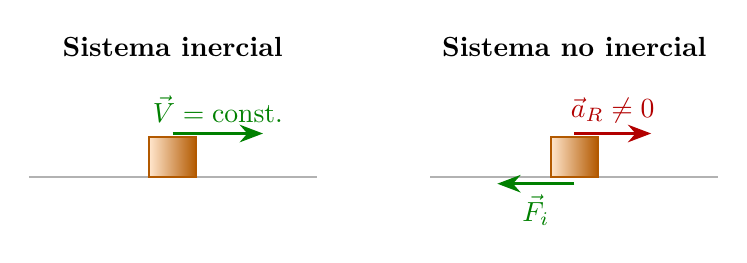
\begin{tikzpicture}[>=Stealth, scale=0.85]

% ---------------- INERCIAL ----------------

\node[
    black,
    font=\bfseries
] at (2.35,2.5) {Sistema inercial};

% Terra
\draw[
    thick,
    gray!60
] (0.2,0.55) -- (4.5,0.55);

% Objecte 3D
\shade[
    shading=axis,
    left color=orange!20,
    right color=orange!70!black
] (2.0,0.55) rectangle (2.7,1.15);

\draw[
    thick,
    orange!70!black
] (2.0,0.55) rectangle (2.7,1.15);

% Velocitat constant
\draw[
    ->,
    very thick,
    green!50!black
] (2.35,1.2) -- (3.7,1.2)
    node[midway, above] {$\vec V=\text{const.}$};


% ---------------- NO INERCIAL ----------------

\node[
    black,
    font=\bfseries
] at (8.35,2.5) {Sistema no inercial};

% Terra
\draw[
    thick,
    gray!60
] (6.2,0.55) -- (10.5,0.55);

% Objecte 3D
\shade[
    shading=axis,
    left color=orange!20,
    right color=orange!70!black
] (8.0,0.55) rectangle (8.7,1.15);

\draw[
    thick,
    orange!70!black
] (8.0,0.55) rectangle (8.7,1.15);

% Acceleració
\draw[
    ->,
    very thick,
    red!70!black
] (8.35,1.2) -- (9.5,1.2)
    node[midway, above] {$\vec a_R\neq0$};

% Força inercial
\draw[
    ->,
    very thick,
    green!50!black
] (8.35,0.45) -- (7.2,0.45)
    node[midway, below] {$\vec F_i$};

\end{tikzpicture}

\end{center}

\begin{demobox}
    Si tenim les coordenades \textbf{R} i \textbf{R'}, un sistema inercial té unes cordenades;

    $ \begin{pmatrix}
\vec{r} = \vec{r'} + \vec{R} \\
\dot{\vec{r}} = \dot{\vec{r'}} + \dot{\vec{R}} \\
\ddot{\vec{r}} =\ddot{\vec{r'}} + \ddot{\vec{R}} 
\end{pmatrix}  $

En els sistemes inercials sabem que $\frac{\vec{F}}{m} = \ddot{\vec{r'}} + \ddot{\vec{R}}$ com que $\ddot{\vec{R}}$ és 0 $\vec{F} = m\ddot{\vec{r'}}= m \ddot{\vec{r}}$
En els sistemes no inercials com que $\ddot{\vec{R}} \neq 0$, obtenim que $\vec{F} -m\ddot{\vec{R}} = m \ddot{\vec{r}}$ on podem anomenar,

\[\text{Força Intercial =} -m \ddot{\vec{R}}\]

De manera que obtenim $\vec{F} + \vec{F_i} = m \ddot{\vec{r}}$
\end{demobox}

\subsection{MCU i MCUA}

Poso el MCU i MCUA dins d'aquesta secció ja que per aquests moviments hem de fer un petit canvi de base a cordenades polars.

\begin{center}
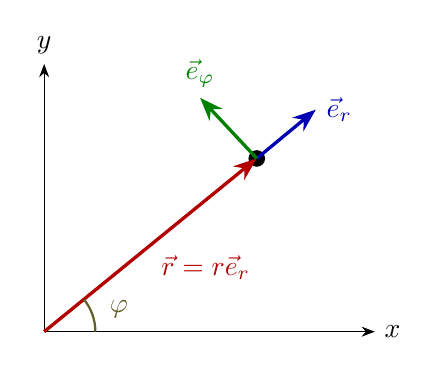
\begin{tikzpicture}[>=Stealth, scale=1]

% Eixos
\draw[->, black] (0,0) -- (4.2,0) node[right] {$x$};
\draw[->, black] (0,0) -- (0,3.4) node[above] {$y$};

% Punt
\fill[black] (2.7,2.2) circle (3pt);

% Radi
\draw[
    ->,
    very thick,
    red!70!black
] (0,0) -- (2.7,2.2)
    node[midway, below right] {$\vec r=r\vec e_r$};

% e_r
\draw[
    ->,
    very thick,
    blue!70!black
] (2.7,2.2) -- (3.45,2.82)
    node[right] {$\vec e_r$};

% e_phi
\draw[
    ->,
    very thick,
    green!50!black
] (2.7,2.2) -- (1.98,2.97)
    node[above] {$\vec e_\varphi$};

% angle
\draw[
    thick,
    olive!60!black
] (0.65,0) arc (0:39:0.65);

\node[olive!60!black] at (0.95,0.28) {$\varphi$};

\end{tikzpicture}
\end{center}

Si en les \textbf{cordenades cartesianes} necesitem \textit{(x,y)}, en les polars necessitem \textit{(r, $\varphi$)}, on r és el mòdul del vector posició i definim que,

$x = r\cos \varphi$

$y = r\sin \varphi$

Com tota base, necesita \textbf{vectors unitaris}, si en la grafica 1 dibuixem els vectors directors, ens surten seguint la linea del vector r i el normal a la linea, definim cadascun com.

$e_x = (\cos \varphi, \sin \varphi)$

$e_\varphi = (-\sin \varphi, \cos \varphi)$

Recordem que per molt que hi hagi una velocitat tangencial que existeixi $v$ es crea una acceleració centripeta de manera que \textbf{es crea una força}.

Podem veure fàcilment que $\vec{e_r}, \vec{e_{\varphi}}$ depenen de $\varphi$ i del temps, de manera que $\dv{}{t}\vec{e_r} = \dot{\varphi} \vec{e_{\varphi}}$ i que $\dv{}{t}\vec{e_{\varphi}} = -\dot{\varphi} \vec{ e_{r}}$ de manera que podem descriure un vector \textbf{$\vec{r} = r\vec{e_r}$} i derivar-lo respecte del temps per \textbf{obtenir la velocitat.}

\begin{demobox}
\[\vec{v} = \dot{\vec{r}} = \dv{}{t}r\vec{e_r} = r \dot{\varphi}\vec{e_\varphi}\]
\[\dot{\varphi} \equiv \omega\]
\end{demobox}

Acabem amb la relació de que $v = r\omega$ i va en direcció \textbf{tangencial al moviment}. Ara, quan apareix un canvi en la velocitat apareix una acceleració, tal i com hem descrit als altres moviments, pero ara com que $\omega$ i $\vec{e_{\varphi}}$ depenen de temps és dona la regla del producte

\begin{center}
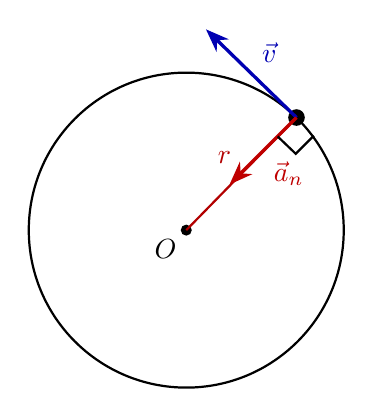
\begin{tikzpicture}[>=Stealth, scale=1]

% Circumferència
\draw[
    thick,
    black
] (0,0) circle (2);

% Centre
\fill (0,0) circle (2pt);
\node[below left] at (0,0) {$O$};

% Punt
\fill[black] (1.4,1.43) circle (3pt);

% Radi
\draw[
    thick,
    red!70!black
] (0,0) -- (1.4,1.43)
    node[midway, above left] {$r$};

% Velocitat
\draw[
    ->,
    very thick,
    blue!70!black
] (1.4,1.43) -- (0.25,2.55)
    node[midway, above right] {$\vec v$};

% Acceleració centrípeta
\draw[
    ->,
    very thick,
    red!75!black
] (1.4,1.43) -- (0.55,0.58)
    node[midway, below right] {$\vec a_n$};

% angle recte
\draw[
    thick
] (1.16,1.19) -- (1.39,0.97) -- (1.62,1.20);

\end{tikzpicture}
\end{center}

\begin{demobox}
    \[\vec{a} = \dot{\vec{v}} = \ddot{\vec{r}} = r\ddot{\varphi}\vec{e_{\varphi}} - r\dot{\varphi}\dot{\varphi} \vec{e_r}\]
    \[\ddot{\varphi} \equiv \alpha\]
\end{demobox}

Per tant tenim dues acceleracions, una que es diu \textbf{tangencial} $a_t = r\alpha$ que va en direcció tangencial a la trajectoria i la \textbf{normal} que va en oposat al vector director $\vec{e_r}$ i que és $a_n = r\omega^2 = \frac{v^2}{r}$.

L'acceleració normal és centripeta i per tant crea una força centripeta al cos.

\subsection{Moviment General en 2D}

Aquí tot i que determinem $\vec{r}(t)$ en les bases cartesianes $\vec{i}, \vec{j}$ despres usem la nostra base propia que canvia en funció del temps amb \textbf{els vectors de frenet} on $e_1$ pren la direcció de la velocitat i l'acceleració tangencial i $e_2$ pren el sentit de l'acceleració normal.

Donat $r(t)$ podem trobar $v(t)$ fàcilment derivant la posció. Amb això podem determinar el nostre \textbf{primer vector de frenet}, de manera que $\vec{e_1} = \frac{\dot{\vec{x}}(t)}{\abs{\dot{\vec{x}}(t)}} = \frac{\vec{v}(t)}{\abs{\vec{v}(t)}}$. I si derivem podem trobar el \textbf{segon vector de frenet}, de manera que; $\vec{e_2} = \frac{\dot{\vec{e_1}}}{\abs{\dot{\vec{e_1}}}}$ ja que han de formar una base;

\begin{center}
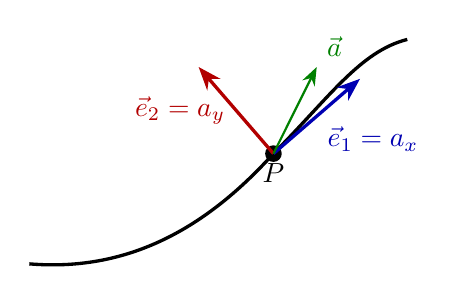
\begin{tikzpicture}[>=Stealth, scale=1]

% Trajectòria corba
\draw[
    very thick,
    black
] (0,0.4)
  .. controls (1.2,0.3) and (2.2,0.8) ..
  (3.1,1.8)
  .. controls (3.8,2.5) and (4.2,3.1) ..
  (4.8,3.25);

% Punt
\fill[black] (3.1,1.8) circle (3pt);

% Tangent e1
\draw[
    ->,
    very thick,
    blue!70!black
] (3.1,1.8) -- (4.2,2.75)
    node[midway, below right] {$\vec e_1 = a_x$};

% Normal e2
\draw[
    ->,
    very thick,
    red!70!black
] (3.1,1.8) -- (2.15,2.9)
    node[midway, left] {$\vec e_2 = a_y$};

% Acceleració
\draw[
    ->,
    thick,
    green!50!black
] (3.1,1.8) -- (3.65,2.9)
    node[above right] {$\vec a$};

\node[below] at (3.1,1.8) {$P$};

\end{tikzpicture}
\end{center}

\begin{demobox}
    \[\abs{\vec{e_1}}^2 = 1\]
    \[\dv{}{t}\abs{\vec{e_1}}^2 = 1  \]
    \[2 \abs{\dot{\vec{e_1}}} \cdot \abs{\vec{e_1}} = 0\]
\end{demobox}

Quan ja tenim la nostra base, per definició donem la velocitat com $\vec{v}(t) = v\vec{e_1}$. I simplement si volem trobar l'acceleració derivem usant la regla de la cadena;

\[\vec{a}(t) = \dot{\vec{v}}(t) = \dot{v}\vec{e_1} + v\dot{\vec{e_1}}\]
\[R = \frac{\vec{v}}{\vec{e_2}}\]
\[\vec{a}(t) = \dot{\vec{v}}(t) = \dot{v}\vec{e_1} + \frac{v^2}{R}{\vec{e_2}}\]

On un altre cop tenim l'acceleració tangencial i l'acceleració normal una apuntant en cada direcció i el mòdul d'aquestes indica l'acceleració del nostre cos.

Denominem K al recíproc del Radi de corbatura, k (en $m^-1$) ens indica com canvia l'angle $\varphi$ respecte de l'elongació, $\frac{\Delta \varphi}{\Delta s}$, si prenem el límit a $\Delta s$ quan s'aproxima a 0, estem mirant l'angle instantani i el canvi d'aquest $k = \abs{\frac{\dv{\varphi}{t}}{\dv{s}{t}}} = \abs{\frac{\dot{\varphi}}{v}}$.

Si ens fixem amb com definim \textbf{els vectors de frenet} en l'espai amb $\varphi$, $\vec{e_1} = \vec{i}\cos \varphi + \vec{j} \sin \varphi$, de manera que $\abs{\vec{e_1}} = \dot{\varphi}$, per tant;

\[\boxed{k = \frac{\abs{\vec{e_1}}}{\abs{\vec{v}}}}, \boxed{R = \frac{\abs{\vec{v}}}{\abs{\vec{e_1}}}}\]

Aquest radi de corbatura normalment s'escriu $R(t)$, ja que com hem vist \textbf{els vectors de frenet depenen del temps} i de la velocitat, si R no canvia estem parlant d'un moviment circular, sinó  el radi canvia i la corbatura també.

\subsection{Distàncies}

Si sabem que $\vec{v} = \dv{\vec{r}}{t}$ doncs quan afegim tots els trossos \textbf{dr} en una integral podem obtenir la distància recorregura $\int_{t_0}^{t} v(t) dt$. 

\begin{center}

\begin{tikzpicture}[>=Stealth, scale=1]

% Trajectòria
\draw[
    very thick,
    black
] (0,0.5)
  .. controls (1,2.7) and (2.5,-0.5) ..
  (4.8,2.6);

% Punt inicial
\fill[black] (0,0.5) circle (3pt);
\node[below left] at (0,0.5) {$P_0$};

% Punt final
\fill[black] (4.8,2.6) circle (3pt);
\node[above right] at (4.8,2.6) {$P$};

% Petit element de longitud d'arc ds
\draw[
    very thick,
    blue!70!black
] (2.20,0.30)
  .. controls (2.32,0.22) and (2.48,0.27) ..
  (2.65,0.39);

% Marques als extrems de ds
\draw[
    thick,
    blue!70!black
] (2.16,1.2) -- (2.24,0.24);

\draw[
    thick,
    blue!70!black
] (2.61,1) -- (2.69,0.33);

% Etiqueta ds
\node[
    blue!70!black,
    fill=white,
    inner sep=2pt
] at (2.43,1.2) {$ds$};

\end{tikzpicture}

\end{center}

Pero que fem quan no ens parlen de temps i ens donen una funció arbitraria? Doncs proposem x = t, de manera que desenvolupant.

\begin{demobox}
    \[\dot{x} = \dv{x}{x} = 1, \dot{y} = \dv{y}{x} = y'\]
    \[\int_{x_0}^{x} \abs{\dot{x}\vec{i} + \dot{y}\vec{j}} = \int_{x_0}^{x} \sqrt{1+y'}\]
\end{demobox}

Per acabar podem distingir magnituds que \textbf{depenen del temps} com;

\begin{itemize}
    \item Vectors de frenet
    \item Velocitat, Posició i Acceleració
    \item Radi
\end{itemize}

Dels que \textbf{no depenen del temps};

\begin{itemize}
    \item Distància de trajectoria
\end{itemize}

\subsection{Casos Particulars}

Aquests són problemes típics o cassos particulars que poden aparèixer al examen i tenen una forma sistemàtica de resoldre

\subsubsection{Politjes}

En un sistema de politjes \textbf{asumim que la longitud $L$ de la corda és constant}, de manera que podem crear un sistema d'equacions amb $s_n \leftrightarrow \Sigma s_n = L$ on relacionem les longituds $s_n$ amb $y_n$ que és la posició de les politjes i que $\dot{y_n} = v_n$ per trobar la relació entre velocitats.

\begin{center}

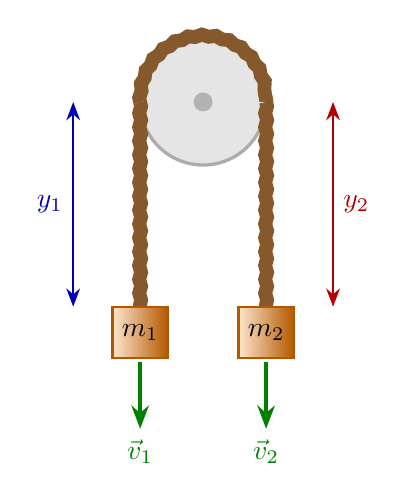
\begin{tikzpicture}[>=Stealth, scale=1]

% ---------------- POLITJA ----------------

% Politja
\fill[gray!20] (3,3.5) circle (0.8);

\draw[
    very thick,
    gray!65
] (3,3.5) circle (0.8);

% Eix central
\fill[gray!60] (3,3.5) circle (0.12);


% ---------------- CORDA ----------------

% Extrem esquerre
\draw[
    line width=5pt,
    brown!70!black,
    decorate,
    decoration={
        snake,
        amplitude=0.35pt,
        segment length=5pt
    }
] (2.2,3.5) -- (2.2,0.9);

% Corda al voltant de la politja
\draw[
    line width=5pt,
    brown!70!black,
    decorate,
    decoration={
        snake,
        amplitude=0.35pt,
        segment length=5pt
    }
] (2.2,3.5)
    arc (180:0:0.8);

% Extrem dret
\draw[
    line width=5pt,
    brown!70!black,
    decorate,
    decoration={
        snake,
        amplitude=0.35pt,
        segment length=5pt
    }
] (3.8,3.5) -- (3.8,0.9);


% ---------------- BLOCS ----------------

% m1
\shade[
    shading=axis,
    left color=orange!20,
    right color=orange!70!black
] (1.85,0.25) rectangle (2.55,0.9);

\draw[
    thick,
    orange!70!black
] (1.85,0.25) rectangle (2.55,0.9);

\node at (2.2,0.575) {$m_1$};


% m2
\shade[
    shading=axis,
    left color=orange!20,
    right color=orange!70!black
] (3.45,0.25) rectangle (4.15,0.9);

\draw[
    thick,
    orange!70!black
] (3.45,0.25) rectangle (4.15,0.9);

\node at (3.8,0.575) {$m_2$};


% ---------------- VELOCITATS ----------------

\draw[
    ->,
    very thick,
    green!50!black
] (2.2,0.2) -- (2.2,-0.65)
    node[below] {$\vec v_1$};

\draw[
    ->,
    very thick,
    green!50!black
] (3.8,0.2) -- (3.8,-0.65)
    node[below] {$\vec v_2$};


% ---------------- ALÇADA ----------------

\draw[
    <->,
    thick,
    blue!70!black
] (1.35,0.9) -- (1.35,3.5)
    node[midway,left] {$y_1$};

\draw[
    <->,
    thick,
    red!70!black
] (4.65,0.9) -- (4.65,3.5)
    node[midway,right] {$y_2$};

\end{tikzpicture}

\end{center}

\[ \dot{y_1} \equiv \mp v_1\]
\[\dot{y_1} \equiv \pm v_2\]

\section{Dinàmica}

Estudia el \textbf{moviment dels objectes}, des de les forçes que el pertorben.

\subsection{Lleis de Newton}

Per poder predir el moviment usem les \textbf{3 lleis de Newton}

\begin{itemize}
    \item \textit{Llei de l'inèrcia}; Un cos en repos no experimenta un canvi si no es pertorbat. 
    \item \textit{Segona Llei}; Una força actua sobre un cos \textbf{otorgant-li acceleració}, $F = m\vec{a}$
    \item \textit{Acció-Reacció}; Si un objecte fa força sobre un altre, aquell altre li fa una contrària en \textbf{sentit oposat}, pero aquesta mai s'aplica si tractem el conjunt com un únic cos perque sinò seria $\Sigma \vec{F} = m\vec{a}$
\end{itemize}

\begin{center}

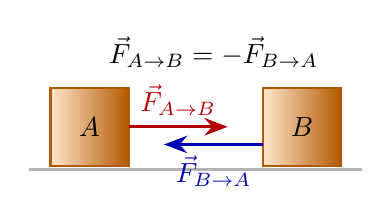
\begin{tikzpicture}[>=Stealth, scale=0.9]

% ---------------- SÒL ----------------

\draw[
    very thick,
    gray!60
] (0.2,0.45) -- (4.9,0.45);


% ---------------- OBJECTES ----------------

% Objecte A
\shade[
    shading=axis,
    left color=orange!20,
    right color=orange!70!black
] (0.5,0.5) rectangle (1.6,1.6);

\draw[
    thick,
    orange!70!black
] (0.5,0.5) rectangle (1.6,1.6);

\node at (1.05,1.05) {$A$};


% Objecte B
\shade[
    shading=axis,
    left color=orange!20,
    right color=orange!70!black
] (3.5,0.5) rectangle (4.6,1.6);

\draw[
    thick,
    orange!70!black
] (3.5,0.5) rectangle (4.6,1.6);

\node at (4.05,1.05) {$B$};


% ---------------- FORCES ----------------

\draw[
    ->,
    very thick,
    red!70!black
] (1.6,1.05) -- (3.0,1.05)
    node[midway, above] {$\vec F_{A\to B}$};

\draw[
    ->,
    very thick,
    blue!70!black
] (3.5,0.8) -- (2.1,0.8)
    node[midway, below] {$\vec F_{B\to A}$};


% ---------------- IGUALTAT ----------------

\node at (2.8,2.1)
    {$\vec F_{A\to B}=-\vec F_{B\to A}$};

\end{tikzpicture}

\end{center}

Sabem que $\vec{F}$ depèn de $\vec{r}(t), \dot{\vec{r}}(t), t$ i que;

\[\frac{\vec{F}(\vec{r}(t), \dot{\vec{r}}(t), t)}{m} = \ddot{\vec{r}}(t)\]

El que realment es vol trobar és la força que pertorba aquell cos i li dona una acceleració, com;

\begin{itemize}
    \item $F = G\frac{Mm}{r^2}$
    \item $F = -k\Delta x$
    \item $F = qvB$
\end{itemize}

\subsection{Forces}

Sobre qualsevol cos pot actuar una força. Si ens trobem a la terra un cos X rep \textbf{un pes} i la terra genera una força en sentit oposat (\textit{tercera llei de Newton}). Però que passa si ens trobem assobre d'una superficie. No caiem cap abaix, això indica \textbf{que existeix una força en reacció a una superficie}. Aquesta és la força normal que és \textit{perpendicular a la superficie de repòs}, aquesta força, naturalment, genera una força' en sentit oposat com a reacció d'aquella. L'acceleració que obté la terra del pes d'un objecte X és infinitéssimament petita per això mai es té en compte.

\[P = P' \leftrightarrow m_T \cdot a_t = m_X \cdot g\]

\begin{center}

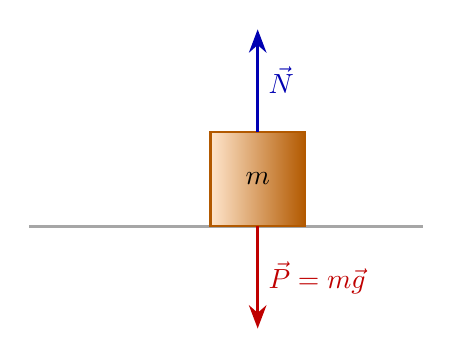
\begin{tikzpicture}[>=Stealth, scale=1]

% Superfície

\draw[
    very thick,
    gray!70
] (-0.5,0) -- (4.5,0);


% Cos

\shade[
    shading=axis,
    left color=orange!20,
    right color=orange!70!black
] (1.8,0) rectangle (3,1.2);

\draw[
    thick,
    orange!70!black
] (1.8,0) rectangle (3,1.2);

\node at (2.4,0.6) {$m$};


% Pes

\draw[
    ->,
    very thick,
    red!75!black
] (2.4,0) -- (2.4,-1.3)
    node[midway, right] {$\vec P=m\vec g$};


% Normal

\draw[
    ->,
    very thick,
    blue!70!black
] (2.4,1.2) -- (2.4,2.5)
    node[midway, right] {$\vec N$};

\end{tikzpicture}

\end{center}
\subsection{Camp Gravitatori}

Si dos objectes qualsevol tenen massa, es genera una força atractiva entre ells amb relació a la seva distància de manera que.

\[\vec{F} = - G\frac{Mm}{r^2} \vec{u_r}\]

On agafa el vector director entre els dos cossos (Cos Origen - Cos Afectat), li dona la volta i ho multiplica per un factor $G\frac{Mm}{r^2}$. També podem obtenir un \textbf{camp vectorial} $g = \frac{\vec{F}}{m}$ on obtenim un conjunt de vectors que al aplicar una massa m obtenen la força de gravitació,

\begin{center}
    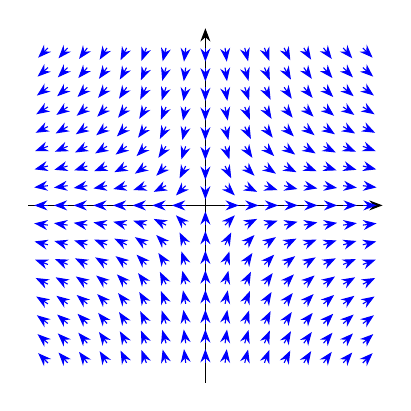
\begin{tikzpicture}[>=Stealth, scale=0.5]

% Ejes
\draw[->] (-4.5,0) -- (4.5,0);
\draw[->] (0,-4.5) -- (0,4.5);

% Campo vectorial
\foreach \x in {-4,-3.5,...,4}{
    \foreach \y in {-4,-3.5,...,4}{
        \pgfmathsetmacro{\r}{sqrt(\x*\x+\y*\y)}
        \ifdim\r pt>0.1pt
            \draw[->,blue]
                (\x,\y) -- 
                ({\x+0.35*\x/\r},{\y-0.35*\y/\r});
        \fi
    }
}

\end{tikzpicture}
\end{center}

\subsubsection{Gravetat Artificial}

Es pot crear un \textbf{pes artficial} si tenim una esfera on el producte $R\omega^2 = g$ que és la força de la gravetat sempre i quant el moviment del observador sigui solidari al de la roda.

Si $R\downarrow, P\downarrow$

Si $\omega \downarrow (\text{ha de}), R \uparrow$

\subsubsection{Cancelació de la Gravetat}

En alguns moments, els efectes de la gravetat $g$ poden semblar indistingibles (\textbf{caiguda lliure}). Segons un teorema la \textit{massa gravitatoria (la massa d'un cos que experimenta la gravetat)} i la \textit{massa inercial (la massa que obté una acceleració)} són les mateixes de manera que en $F = ma = G\frac{Mm}{r^2}$ es simplifiquen i obtenim $\vec{a} = -G\frac{M}{r^2} \vec{u_r}$

De manera que \textbf{la massa no influeix}, quan diem "cancelar la gravetat" ens referim a estar en una situació de \textbf{caiguda lliure} on $a = g$ de manera que tot cau en sincronització a la gravetat i $F + N = mg$, $N = mg - mg = 0$ no hi ha recolzament del terra i segons el sistema $a = 0$ i \textit{els objectes floten}

\begin{center}

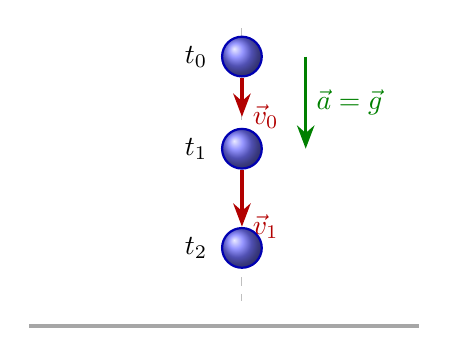
\begin{tikzpicture}[>=Stealth, scale=0.9]

% Terra
\draw[
    very thick,
    gray!70
] (-0.5,0) -- (5,0);

% Trajectòria
\draw[
    dashed,
    gray!50
] (2.5,4.2) -- (2.5,0.35);


% Posició inicial
\shade[
    shading=ball,
    ball color=blue!55
] (2.5,3.8) circle (0.28);

\draw[
    thick,
    blue!70!black
] (2.5,3.8) circle (0.28);

\node[left] at (2.15,3.8) {$t_0$};


% Posició intermèdia
\shade[
    shading=ball,
    ball color=blue!55
] (2.5,2.5) circle (0.28);

\draw[
    thick,
    blue!70!black
] (2.5,2.5) circle (0.28);

\node[left] at (2.15,2.5) {$t_1$};


% Posició final
\shade[
    shading=ball,
    ball color=blue!55
] (2.5,1.1) circle (0.28);

\draw[
    thick,
    blue!70!black
] (2.5,1.1) circle (0.28);

\node[left] at (2.15,1.1) {$t_2$};


% Velocitat inicial
\draw[
    ->,
    very thick,
    red!70!black
] (2.5,3.5) -- (2.5,2.95)
    node[right] {$\vec v_0$};


% Velocitat intermèdia
\draw[
    ->,
    very thick,
    red!70!black
] (2.5,2.2) -- (2.5,1.4)
    node[right] {$\vec v_1$};


% Acceleració
\draw[
    ->,
    very thick,
    green!50!black
] (3.4,3.8) -- (3.4,2.5)
    node[midway,right] {$\vec a=\vec g$};

\end{tikzpicture}

\end{center}

\subsection{Forces de Fregament}

En qualevol cos que es mou \textbf{sobre una superficie}. Com que les superficies mai són completament regulars, experimenta \textit{una restricció} alhora de moure's. Si dibuixem la força de fregament en sentit oposat no vol dir que es mou la contrari, ja que \textbf{és proporcional a la força que fa moure l'objecte}, si no hi ha força no hi ha força de fregament.

S'ha vist que $F_f \propto F_N$ de manera que;

\[F_f = \mu_{e/d}N\]

\begin{center}

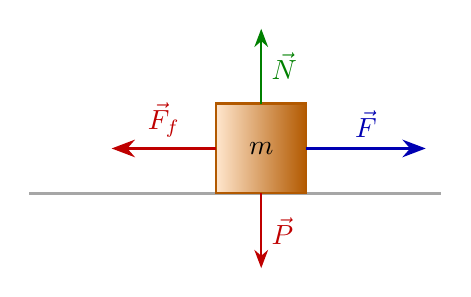
\begin{tikzpicture}[>=Stealth, scale=0.95]

% Superfície

\draw[
    very thick,
    gray!70
] (-0.5,0) -- (5,0);


% Cos

\shade[
    shading=axis,
    left color=orange!20,
    right color=orange!70!black
] (2,0) rectangle (3.2,1.2);

\draw[
    thick,
    orange!70!black
] (2,0) rectangle (3.2,1.2);

\node at (2.6,0.6) {$m$};


% Força aplicada

\draw[
    ->,
    very thick,
    blue!70!black
] (3.2,0.6) -- (4.8,0.6)
    node[midway, above] {$\vec F$};


% Fregament

\draw[
    ->,
    very thick,
    red!75!black
] (2,0.6) -- (0.6,0.6)
    node[midway, above] {$\vec F_f$};


% Normal

\draw[
    ->,
    thick,
    green!50!black
] (2.6,1.2) -- (2.6,2.2)
    node[midway, right] {$\vec N$};


% Pes

\draw[
    ->,
    thick,
    red!75!black
] (2.6,0) -- (2.6,-1)
    node[midway, right] {$\vec P$};

\end{tikzpicture}

\end{center}

Sabem que $\mu_e, \mu_d \exists$ i que $\mu_e > \mu_d$. On definim $\mu_e$ com a \textit{coeficient estàtic} i $\mu_d$ com a \textit{coeficient dinàmic}

\subsection{Casos Particulars}

En aquests apartats estudiarem els \textbf{cassos particulars que ens podem trobar en mecànica}.

\subsubsection{Cordes Ideals}

Anomenem \textit{corda ideal a aquella corda tensionada que té $\Delta m\approx 0$}. Podem demostrar que aquesta força transporta la mateixa tensió en tots els seus punts $ds$.

\begin{demobox}
    Si tenim una corda de llargada \textbf{L} i ho separem en troços petits on estiren 2 tensions obtenim que $T - T' = \Delta m\cdot a$ per tant;
    
    \begin{center}
        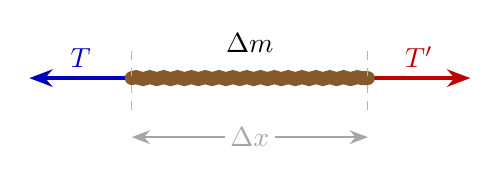
\begin{tikzpicture}[>=Stealth, scale=1]

    \draw[
        line width=5pt,
        brown!70!black,
        decorate,
        decoration={
            snake,
            amplitude=0.35pt,
            segment length=5pt
        }
    ] (1.5,2) -- (4.5,2);

    \draw[
        ->,
        very thick,
        blue!75!black
    ] (1.5,2) -- (0.2,2)
    node[midway, above] {\color{blue!75!black}$T$};

    \draw[
        ->,
        very thick,
        red!75!black
    ] (4.5,2) -- (5.8,2)
    node[midway, above] {\color{red!75!black}$T'$};

    \fill[brown!70!black] (1.5,2) circle (2.5pt);
    \fill[brown!70!black] (4.5,2) circle (2.5pt);

    \draw[
        <->,
        thick,
        gray!70
    ] (1.5,1.25) -- (4.5,1.25)
    node[midway, fill=white, inner sep=2pt] {$\Delta x$};

    \node[
        fill=white,
        inner sep=2pt
    ] at (3,2.45) {$\Delta m$};

    \draw[
        dashed,
        gray!60
    ] (1.5,1.6) -- (1.5,2.4);

    \draw[
        dashed,
        gray!60
    ] (4.5,1.6) -- (4.5,2.4);

\end{tikzpicture}
    \end{center}

    $T-T' = 0a \therefore T = T'$ i així demostm la propietat.
\end{demobox}

Recordar que en tensions \textbf{per la 3ª llei de Newton}, tota tensió té una altra al altre extrem de la corda i una que fa sobre la superficie de la mateixa magnitud que anomenem $F_s$.

\subsubsection{Politjes}

En tot sistema de politjes com hem demostrat abans esta fet amb \textbf{cordes ideals}, mentre no sigui una corda diferent. I que en cada politja podem diferenciar \textbf{força d'entrada ($F_i$)} i \textbf{força de sortida ($F_f$)} on obtenim que $F_i = 2F_f$ per cada politja on entra 1 força i en surten dues.

\subsubsection{Rodes}

Podem diferenciar 2 situacions d'una roda;

\begin{itemize}
    \item \textbf{No Llisca};
    \item \textbf{Llisca};
\end{itemize}

\section{Dinàmica dels Sistemes de Partícules I}

\subsection{Estàtica de Sòlids}

En un inici les lleis de Newton estan formulades \textbf{per punts al espai en 0D}, pero com és que ho apliquem a un conjunt de punts \textbf{0D} que formen un $\R^3$?

\subsection{Moment Lineal}

Considerem una particula de massa $m$ amb velocitat $\vec{v}$ i es pot definit el \textbf{moment lineal com}; $\vec{p} = m\vec{v}$;

\begin{demobox}
    Segons la 3ª Llei de Newton; $\vec{f} = m\vec{a} = m \dv{\vec{v}}{t} = \dv{m\vec{v}}{t} = \dv{\vec{p}}{t} $

    De manera que definim \textbf{la força com a la derivada del moment lineal}.
\end{demobox}

Ara bé, com és que en la llei de Newton mai posem les forçes entre els cossos si parlem del sistema total?

Considerem \textbf{un sistema de particules}; $\vec{P} = \vec{p_1}+ \dots + \vec{p_n}$

\begin{center}
    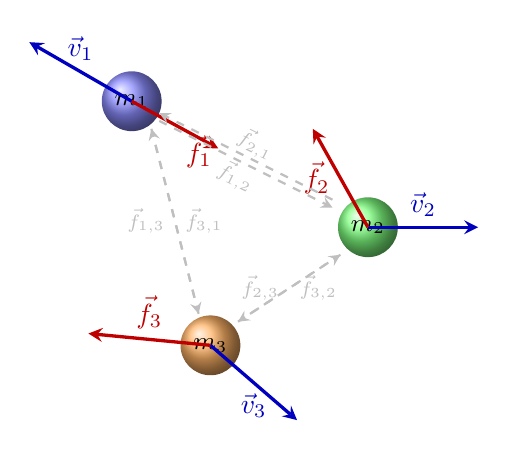
\begin{tikzpicture}[
    >=stealth,
    thick
]

    % Bola
    \shade[
        ball color=blue!45
    ] (1.8,3.6) circle (0.38);

    % Massa
    \node at (1.8,3.6) {\small $m_1$};

    % Velocitat v1
    \draw[
        ->,
        very thick,
        blue!75!black
    ] (1.8,3.6) -- (0.5,4.35)
        node[midway, above] {\color{blue!75!black}$\vec v_1$};

    % Força f1
    \draw[
        ->,
        very thick,
        red!75!black
    ] (1.8,3.6) -- (2.9,3.0)
        node[midway, below right] {\color{red!75!black}$\vec f_1$};

    % Bola
    \shade[
        ball color=green!50
    ] (4.8,2.0) circle (0.38);

    % Massa
    \node at (4.8,2.0) {\small $m_2$};

    % Velocitat v2
    \draw[
        ->,
        very thick,
        blue!75!black
    ] (4.8,2.0) -- (6.2,2.0)
        node[midway, above] {\color{blue!75!black}$\vec v_2$};

    % Força f2
    \draw[
        ->,
        very thick,
        red!75!black
    ] (4.8,2.0) -- (4.1,3.25)
        node[midway, left] {\color{red!75!black}$\vec f_2$};

    % Bola
    \shade[
        ball color=orange!60
    ] (2.8,0.5) circle (0.38);

    % Massa
    \node at (2.8,0.5) {\small $m_3$};

    % Velocitat v3
    \draw[
        ->,
        very thick,
        blue!75!black
    ] (2.8,0.5) -- (3.9,-0.45)
        node[midway, below] {\color{blue!75!black}$\vec v_3$};

    % Força f3
    \draw[
        ->,
        very thick,
        red!75!black
    ] (2.8,0.5) -- (1.25,0.65)
        node[midway, above] {\color{red!75!black}$\vec f_3$};

    % f_12 i f_21
    \draw[
        ->,
        dashed,
        gray!50
    ] (2.15,3.35) -- (4.35,2.25)
        node[midway, above, sloped] {\scriptsize $\vec f_{2,1}$};

    \draw[
        ->,
        dashed,
        gray!50
    ] (4.35,2.35) -- (2.15,3.45)
        node[midway, below, sloped] {\scriptsize $\vec f_{1,2}$};

    % f_13 i f_31
    \draw[
        ->,
        dashed,
        gray!50
    ] (2.05,3.25) -- (2.65,0.9)
        node[midway, right] {\scriptsize $\vec f_{3,1}$};

    \draw[
        ->,
        dashed,
        gray!50
    ] (2.65,0.9) -- (2.05,3.25)
        node[midway, left] {\scriptsize $\vec f_{1,3}$};

    % f_23 i f_32
    \draw[
        ->,
        dashed,
        gray!50
    ] (4.45,1.65) -- (3.15,0.8)
        node[midway, right] {\scriptsize $\vec f_{3,2}$};

    \draw[
        ->,
        dashed,
        gray!50
    ] (3.15,0.8) -- (4.45,1.65)
        node[midway, left] {\scriptsize $\vec f_{2,3}$};

\end{tikzpicture}
\end{center}

Pel teorema $\dv{\vec{P}}{t} = \vec{F} = \vec{f_1} + \dots + \vec{f_n}$. Com que estem contant el sistema com un total, \textbf{les forçes internes $\vec{f_{1,2}}, \vec{f_{2,1}}, \vec{f_{1,3}}, \vec{f_{3,1}}, \vec{f_{2,3}}, \vec{f_{3,2}}$} es cancelen ja que són idèntiques en sentits oposats.

\subsection{Centre de Masses}

Anomenem centre de masses d'un sistema $M = (m_1, \dots, m_n)$. El centre de masses és una \textbf{mitjana ponderada} dels vectors posició de totes les particules;

\[\vec{R_t}= \frac{\vec{r_1} + \dots + \vec{r_n}}{n}\]

I descrivim el sistema com a $\vec{P} = M\dot{\vec{R}}$ i $\vec{F} = M \ddot{\vec{R}}$

\section{Dinàmica dels Sistemes de Partícules II}

\end{document}